\setlength{\columnsep}{3pt}
\begin{flushleft}
	\bigskip
	To login to any UNIX machine, you need a user. There are 3 types of users in Linux:

	\begin{figure}[h!]
		\centering
		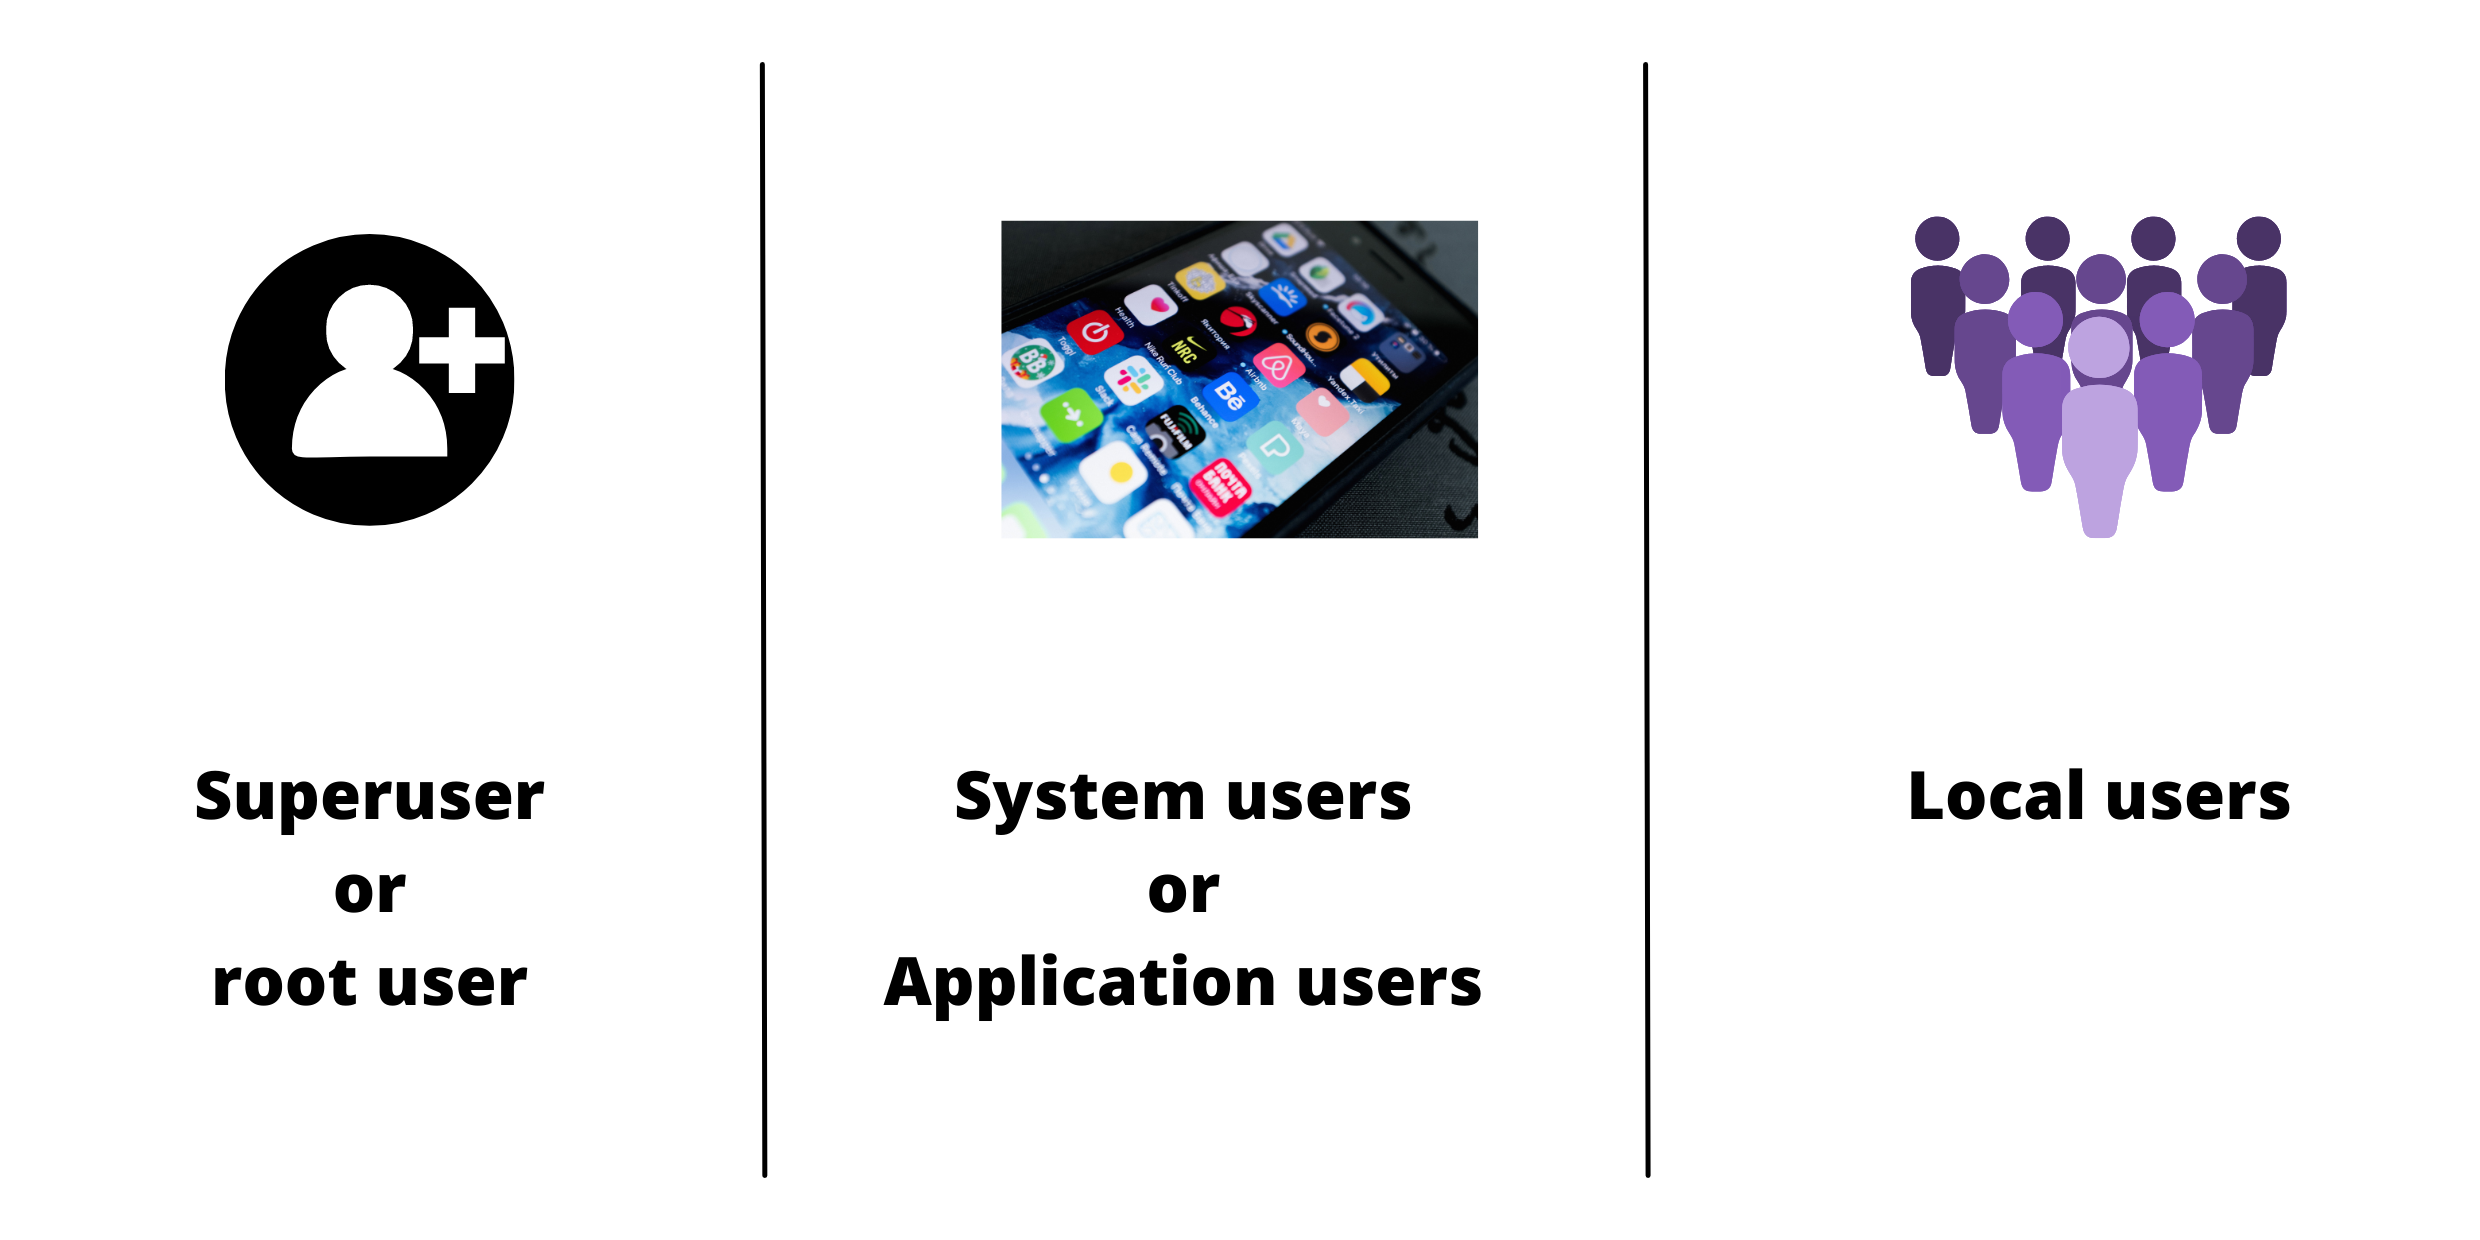
\includegraphics[scale=0.20]{content/chapter4/images/users.png}
		\caption{User types}
		\label{fig:user}
	\end{figure}

	
	\begin{itemize}
		\item \textbf{Superuser i.e. root}: 
		\begin{itemize}
			\item Automatically created when you install Linux.
			\item Superuser can execute commands under \textbf{/usr/sbin \& /usr/bin}.
		\end{itemize}

		\item \textbf{System users}:
		\begin{itemize}
			\item Created automatically during application or software installation.
			\item Eg: When you install VLC media player in Linux, a user named "vlc" will be created automatically.
			\item These accounts exist to allow different services to interact with
			your computer.
		\end{itemize}
		
		\item \textbf{Normal or Local users}:
		\begin{itemize}
			\item Created by root or sudo user.
			\item Local user can execute commands under \textbf{/usr/bin}.
			\item Eg: jack, jill, ram, ravi etc.
		\end{itemize}
		
	\end{itemize}

\end{flushleft}

\newpage





